This problem simulates the interface between a void region and a strong, pure absorber
region, with an incoming flux boundary condition applied.
Table \ref{tab:void_to_absorber} summarizes the problem parameters.

%-------------------------------------------------------------------------------
\begin{table}[htb]\caption{Normal Void-to-Absorber Test Problem Summary}
\label{tab:void_to_absorber}
\centering
\begin{tabular}{l l}\toprule
\emph{Parameter} & \emph{Value}\\\midrule
Domain & $\mathcal{D} = (0,1)^d$\\
Initial Conditions & $u_0(\x)=0$\\
Boundary Conditions & $u(\x,t)=1,\quad \x\in\partial\mathcal{D}^-,\quad t>0$,\\
   & $\quad\partial\mathcal{D}^-=\{\x\in\partial\mathcal{D}:\mathbf{n}(\x)
       \cdot\mathbf{\Omega}<0\}$\\
Direction & $\mathbf{\Omega} = \mathbf{e}_x$\\
Cross Section & $\sigma(\x)=\left\{\begin{array}{c l}
   10, & \x\in(\frac{1}{2},1)^d\\
   0,  & \mbox{otherwise}\end{array}\right.$\\
Source & $q(\x,t)=0$\\
Speed & $\speed=1$\\
Exact Solution & $u(\x,t)=\left\{\begin{array}{l l}
   \scalarsolution_{\text{ss}}(\x), & x-t<0\\
   0, & \mbox{otherwise}
   \end{array}\right.$ \\
   & $\scalarsolution_{\text{ss}}(\x) =
       \left\{\begin{array}{l l}
          e^{-10(x-\frac{1}{2})}, & x\ge\frac{1}{2}, y\ge\frac{1}{2}, z\ge\frac{1}{2}\\
          1,                      & \mbox{otherwise}
       \end{array}\right.$\\
\bottomrule\end{tabular}
\end{table}
%-------------------------------------------------------------------------------

Table \ref{tab:void_to_absorber_run_parameters} shows the run parameters used
to obtain the results in this section, Figures \ref{fig:void_to_absorber_2D_fe}
and \ref{fig:void_to_absorber_2D_ssprk33} show 2-D results for explicit Euler
and SSPRK33 time discretizations, respectively, and Figure
\ref{fig:void_to_absorber_3D} shows 3-D results.

From Figure \ref{fig:void_to_absorber_2D_ssprk33}, one can see that the
Galerkin scheme (which has no artificial dissipation) generates significant
spurious oscillations perpindicular to the transport direction, even below the
absorber region. The oscillations are particularly severe along the lower edge
of the absorber region, where particles/photons are travelling parallel to the
absorber; this edge has a sharper gradient in the solution than the left edge
of the absorber region due to the lack of attenuation in this direction, which
is present for the left edge. Figure \ref{fig:void_to_absorber_2D_ssprk33},
which uses explicit Euler instead of SSPRK33 does not show the Galerkin plot
because the oscillations grew without bound, leading to infinite solution
values. The entropy viscosity scheme is also vulnerable to spurious
oscillations, although to a lesser extent than the Galerkin scheme.

Note that all numerical schemes except the Galerkin scheme involve some
dissipation; this can be seen at the outgoing (right) boundary of the void
region, where there is a solution gradient despite the lack of
absorption. This is because the simulation was run to $t=1$, and the transport
speed is $\speed=1$, so the wave front should be located at the right
boundary of the domain since the domain width is equal to 1;
the diffusivity at the right boundary is due to artificial diffusion
along the wave front.
For steady-state computations, where there is no transient and
thus no wave front, one would not see this diffusivity
at the right boundary.

Figure \ref{fig:void_to_absorber_visc} shows the low-order and entropy
viscosity profiles using SSPRK33, both on linear scales but separately
scaled. One can see that the entropy viscosity
is highest along the incident edge of the absorber region, and in
particular, the corner of the absorber region in the center of the
domain.

One can visually compare the width of the diffusive region to infer the
diffusivity of each numerical scheme. For example, one can see that the
low-order solution is a bit more diffusive than the high-order schemes and FCT
schemes.  Both the Galerkin-FCT and EV-FCT solutions show a lack of
oscillations and less diffusivity than the low-order solution.

The 3-D results are included here to show a proof of principle
that the FCT algorithm used is not restricted to 1-D or 2-D.

%-------------------------------------------------------------------------------
\begin{table}[ht]\caption{Normal Void-to-Absorber Test Problem Run Parameters}
\label{tab:void_to_absorber_run_parameters}
\centering
\begin{tabular}{l l}\toprule
\emph{Parameter} & \emph{Value}\\\midrule
Number of Cells & $N_{cell} = 16384$\\
End Time & $t = 1$\\
CFL Number & $\nu = 0.5$\\\midrule
Entropy Function & $\entropy(\scalarsolution) = \frac{1}{2}\scalarsolution^2$\\
Entropy Residual Coefficient & $\entropyresidualcoef = 0.1$\\
Entropy Jump Coefficient & $\entropyjumpcoef = 0.1$\\
\bottomrule\end{tabular}
\end{table}
%-------------------------------------------------------------------------------
\begin{figure}[ht]
   \centering
   \begin{subfigure}{0.3\textwidth}
      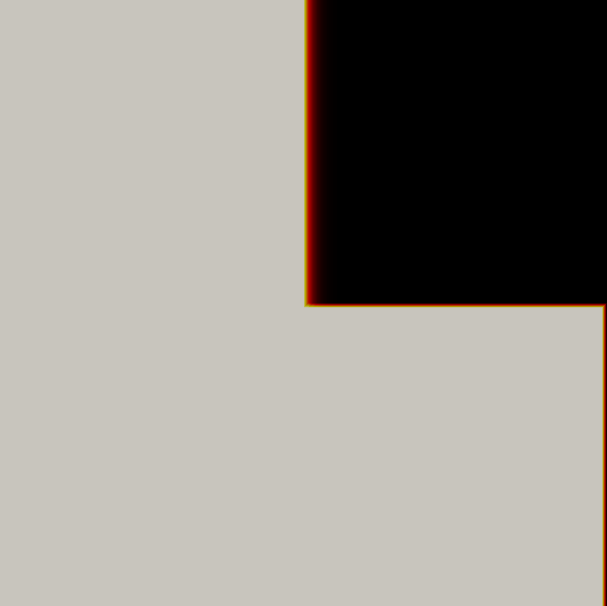
\includegraphics[width=\textwidth]
        {\contentdir/results/transport/void_to_absorber/images/Exact.png}
      \caption{Exact}
   \end{subfigure}
   \begin{subfigure}{0.3\textwidth}
      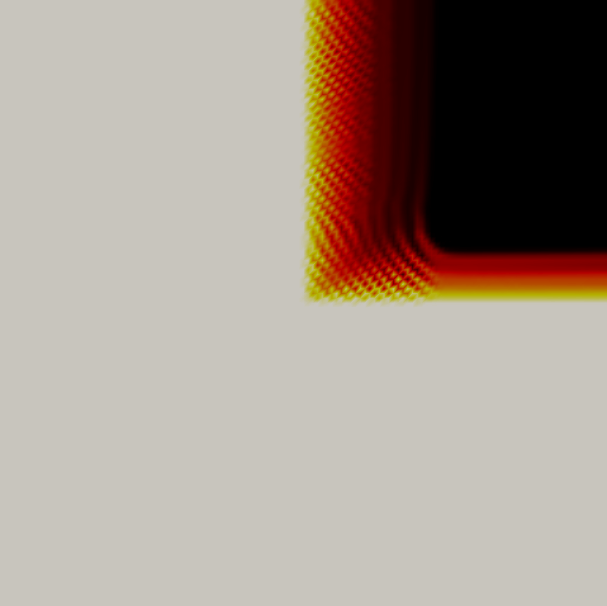
\includegraphics[width=\textwidth]
        {\contentdir/results/transport/void_to_absorber/images/GalFCT_FE.png}
      \caption{Galerkin FCT}
   \end{subfigure}
   \begin{subfigure}{0.3\textwidth}
      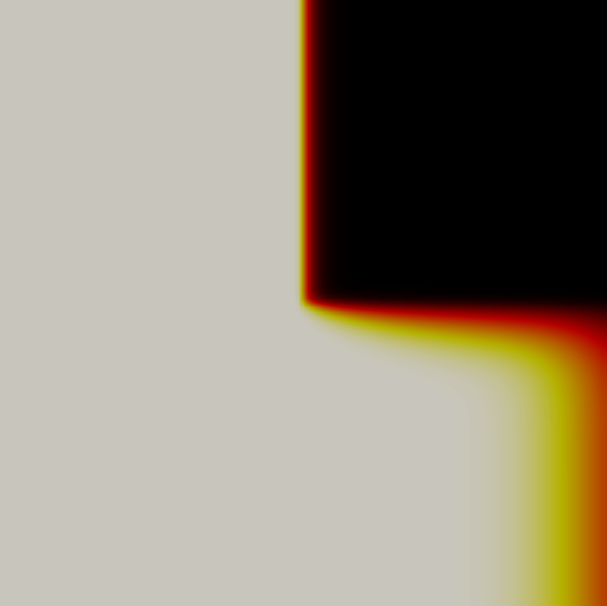
\includegraphics[width=\textwidth]
        {\contentdir/results/transport/void_to_absorber/images/Low_FE.png}
      \caption{Low-Order}
   \end{subfigure}
   \begin{subfigure}{0.3\textwidth}
      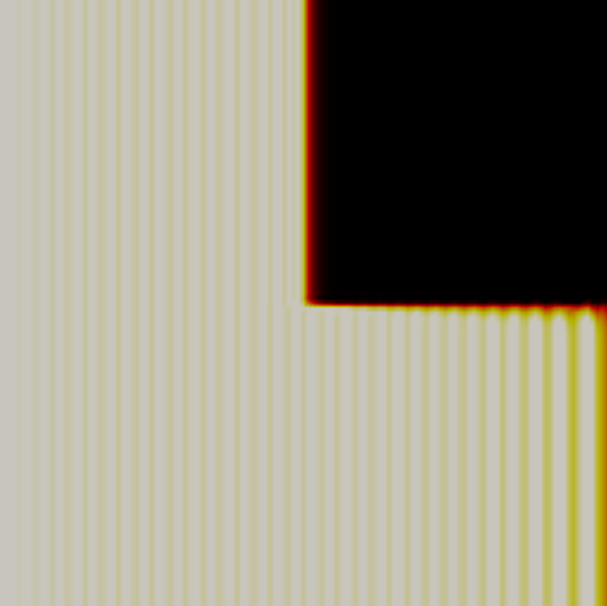
\includegraphics[width=\textwidth]
        {\contentdir/results/transport/void_to_absorber/images/EV_FE.png}
      \caption{Entropy Viscosity}
   \end{subfigure}
   \begin{subfigure}{0.3\textwidth}
      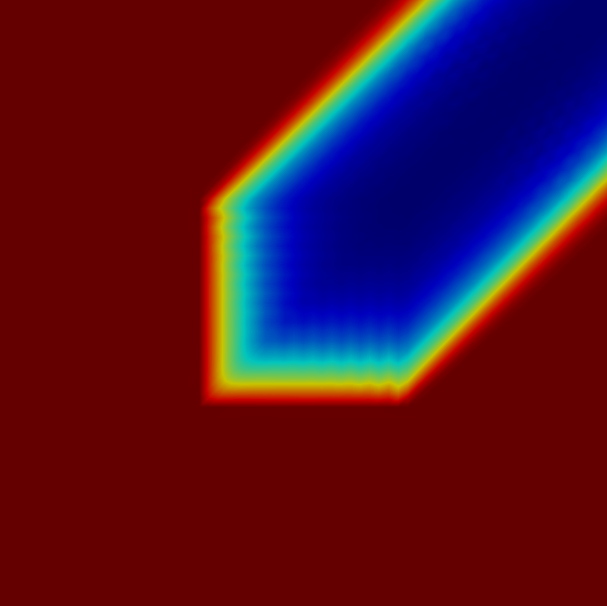
\includegraphics[width=\textwidth]
        {\contentdir/results/transport/void_to_absorber/images/EVFCT_FE.png}
      \caption{Entropy Viscosity FCT}
   \end{subfigure}
   \caption{Comparison of Solutions for 2-D Normal Void-to-Absorber Test
     Problem Using Explicit Euler Time Discretization}
   \label{fig:void_to_absorber_2D_fe}
\end{figure}
%-------------------------------------------------------------------------------
\begin{figure}[ht]
   \centering
   \begin{subfigure}{0.3\textwidth}
      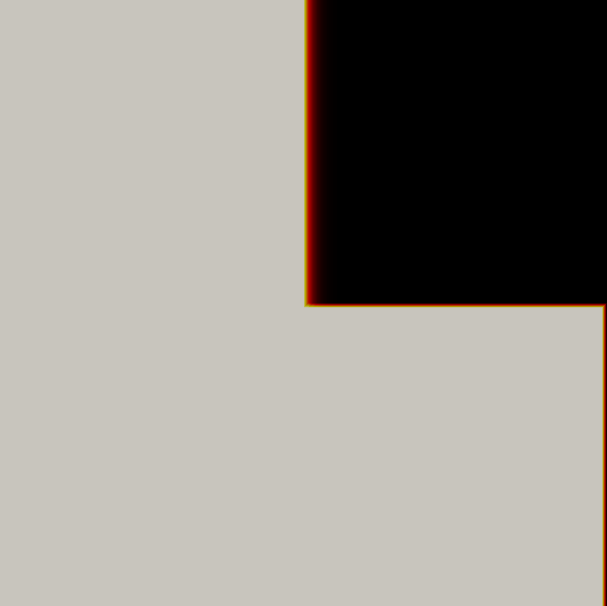
\includegraphics[width=\textwidth]
        {\contentdir/results/transport/void_to_absorber/images/Exact.png}
      \caption{Exact}
   \end{subfigure}
   \begin{subfigure}{0.3\textwidth}
      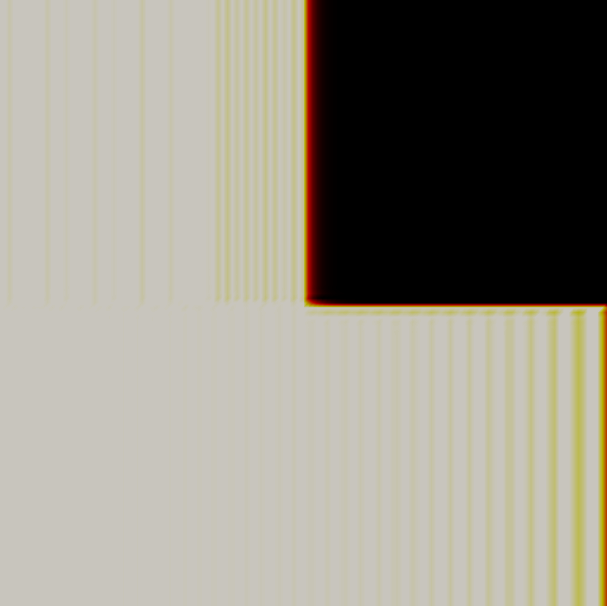
\includegraphics[width=\textwidth]
        {\contentdir/results/transport/void_to_absorber/images/Gal_SSPRK33.png}
      \caption{Galerkin}
   \end{subfigure}
   \begin{subfigure}{0.3\textwidth}
      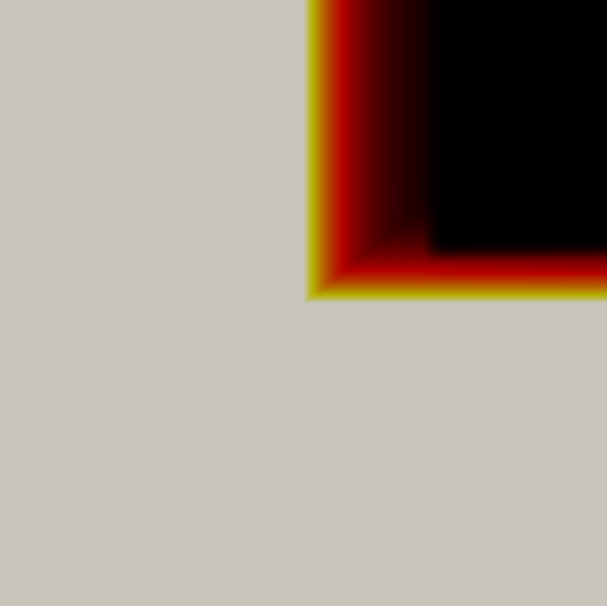
\includegraphics[width=\textwidth]
        {\contentdir/results/transport/void_to_absorber/images/GalFCT_SSPRK33.png}
      \caption{Galerkin FCT}
   \end{subfigure}
   \begin{subfigure}{0.3\textwidth}
      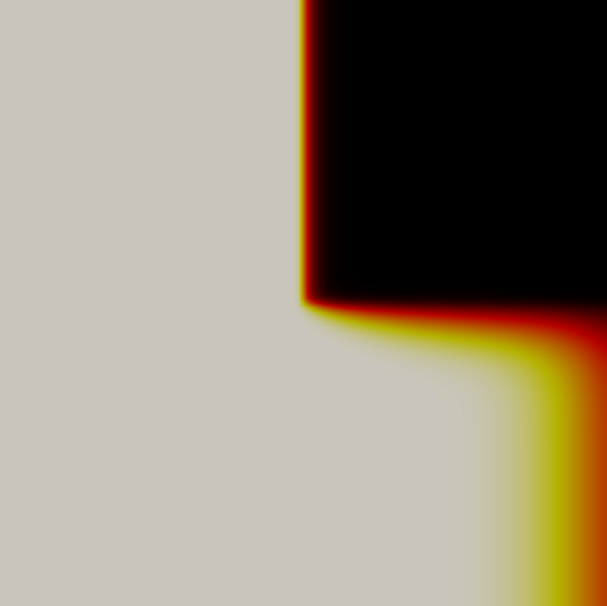
\includegraphics[width=\textwidth]
        {\contentdir/results/transport/void_to_absorber/images/Low_SSPRK33.png}
      \caption{Low-Order}
   \end{subfigure}
   \begin{subfigure}{0.3\textwidth}
      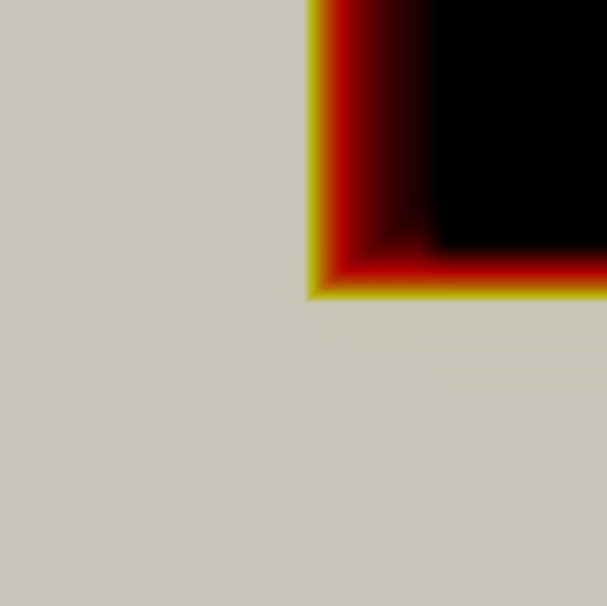
\includegraphics[width=\textwidth]
        {\contentdir/results/transport/void_to_absorber/images/EV_SSPRK33.png}
      \caption{Entropy Viscosity}
   \end{subfigure}
   \begin{subfigure}{0.3\textwidth}
      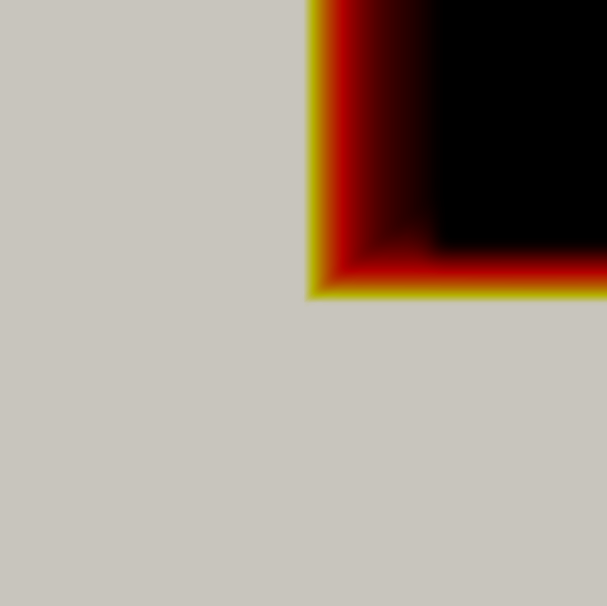
\includegraphics[width=\textwidth]
        {\contentdir/results/transport/void_to_absorber/images/EVFCT_SSPRK33.png}
      \caption{Entropy Viscosity FCT}
   \end{subfigure}
   \caption{Comparison of Solutions for 2-D Normal Void-to-Absorber Test
     Problem Using SSPRK33 Time Discretization}
   \label{fig:void_to_absorber_2D_ssprk33}
\end{figure}
%-------------------------------------------------------------------------------
\begin{figure}[ht]
   \centering
   \begin{subfigure}{0.45\textwidth}
      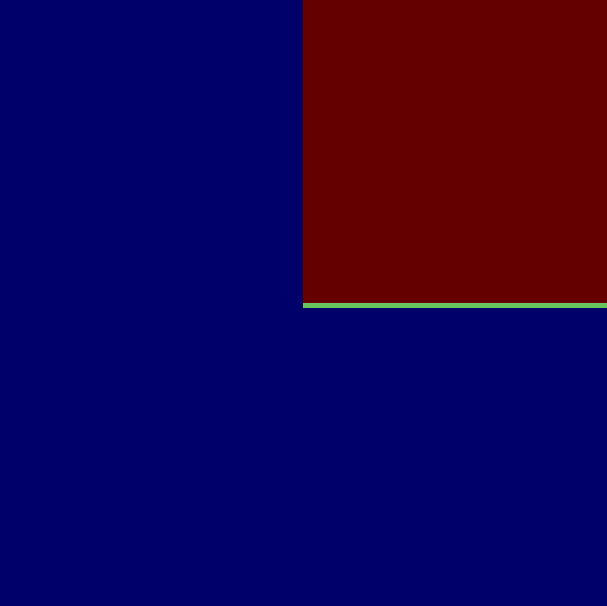
\includegraphics[width=\textwidth]
        {\contentdir/results/transport/void_to_absorber/images/low_viscosity_SSP3_linearscale.png}
      \caption{Low-order viscosity}
   \end{subfigure}
   \begin{subfigure}{0.45\textwidth}
      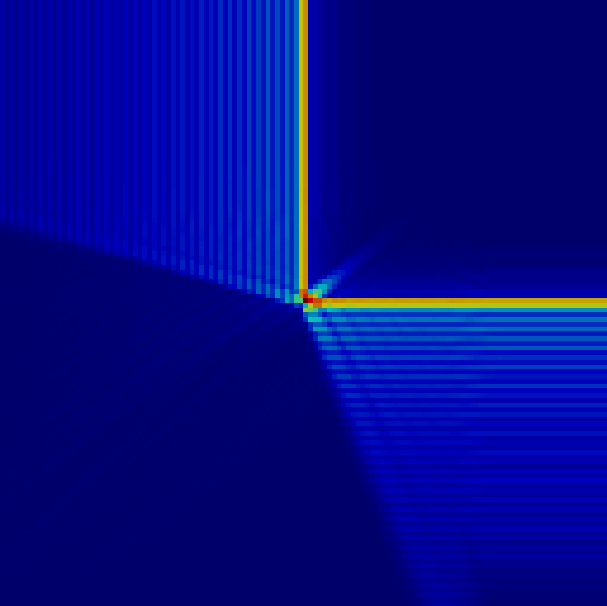
\includegraphics[width=\textwidth]
        {\contentdir/results/transport/void_to_absorber/images/entropy_viscosity_SSP3_linearscale.png}
      \caption{Entropy viscosity}
   \end{subfigure}
   \caption{Viscosity Profiles for the 2-D Void-to-Absorber Test
     Problem Using SSPRK33 Time Discretization}
   \label{fig:void_to_absorber_visc}
\end{figure}
%-------------------------------------------------------------------------------
\begin{figure}[ht]
   \centering
   \begin{subfigure}{0.45\textwidth}
      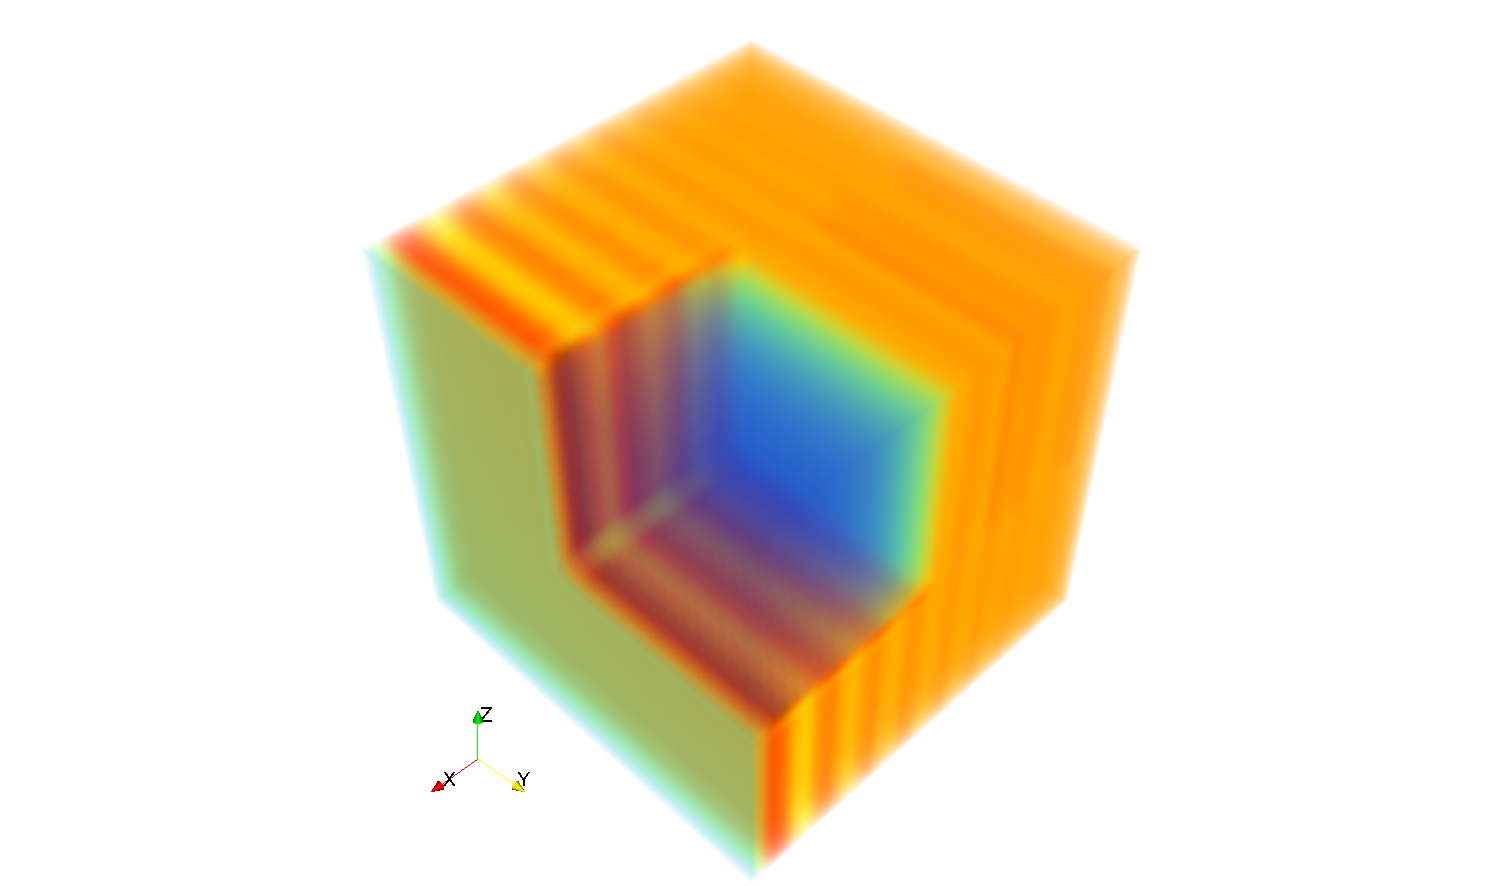
\includegraphics[width=\textwidth]
        {\contentdir/results/transport/void_to_absorber/images/Gal_3D.png}
      \caption{Galerkin}
   \end{subfigure}
   \begin{subfigure}{0.45\textwidth}
      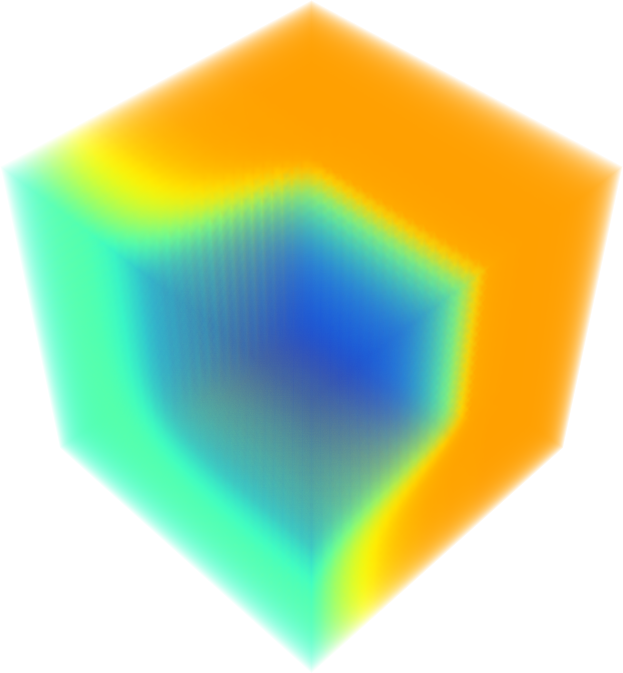
\includegraphics[width=\textwidth]
        {\contentdir/results/transport/void_to_absorber/images/GalFCT_3D.png}
      \caption{Galerkin with FCT}
   \end{subfigure}
   \caption{Comparison of Solutions for the 3-D Normal Void-to-Absorber Test
     Problem Using SSPRK33 Time Discretization}
   \label{fig:void_to_absorber_3D}
\end{figure}
%-------------------------------------------------------------------------------

\clearpage
